%
% Annual Cognitive Science Conference
% Sample LaTeX Paper -- Proceedings Format
%

% Original : Ashwin Ram (ashwin@cc.gatech.edu)       04/01/1994
% Modified : Johanna Moore (jmoore@cs.pitt.edu)      03/17/1995
% Modified : David Noelle (noelle@ucsd.edu)          03/15/1996
% Modified : Pat Langley (langley@cs.stanford.edu)   01/26/1997
% Latex2e corrections by Ramin Charles Nakisa        01/28/1997
% Modified : Tina Eliassi-Rad (eliassi@cs.wisc.edu)  01/31/1998
% Modified : Trisha Yannuzzi (trisha@ircs.upenn.edu) 12/28/1999 (in process)
% Modified : Mary Ellen Foster (M.E.Foster@ed.ac.uk) 12/11/2000
% Modified : Ken Forbus                              01/23/2004
% Modified : Eli M. Silk (esilk@pitt.edu)            05/24/2005
% Modified : Niels Taatgen (taatgen@cmu.edu)         10/24/2006
% Modified : David Noelle (dnoelle@ucmerced.edu)     11/19/2014

%% Change "letterpaper" in the following line to "a4paper" if you must.

\documentclass[10pt,letterpaper]{article}

\usepackage{cogsci}
\usepackage{pslatex}
\usepackage{apacite}

% New command: footnote without reference
\newcommand\blfootnote[1]{%
  \begingroup
  \renewcommand\thefootnote{}\footnote{#1}%
  \addtocounter{footnote}{-1}%
  \endgroup
}


\title{Learning Inductive Biases with Neural Networks}

\author{{\large \bf Reuben Feinman (reuben.feinman@nyu.edu)} \\
  Center for Neural Science \\
  New York University
  \AND {\large \bf Brenden M. Lake (brenden@nyu.edu)} \\
  Department of Psychology and Center for Data Science \\
  New York University}


\begin{document}

\maketitle


\begin{abstract}
    People use rich prior knowledge about the world in order
to efficiently learn new concepts. These priors--commonly referred to as
``inductive biases"--pertain to the space of internal models considered by a
learner, and they help maximize the amount of information that is extracted
from limited data. Recently, it was shown that performance-optimized
deep neural networks (DNNs) develop inductive biases similar to those
possessed by human children. However, these models use unrealistic training
data, and it remains unclear whether they develop their biases in the same way
as humans. We investigate the development and influence of inductive biases
in DNNs using an experimental paradigm borrowed from develpmental psychology.
We find that simple neural network models can develop inductive
biases from as few as 2 examples of each concept, and that these biases tend
to grow with depth in the network. The development of these biases predicts
the onset of vocabulary acceleration in our networks, a finding that mimicks
human children.

\textbf{Keywords:}
learning-to-learn; neural networks; inductive biases
\end{abstract}

\section{Introduction}

Humans possess the remarkable ability to learn a new concept from seeing just a
few examples. A child who is learning her first few words can easily pick up
the meaning of the word ``fork" after observing only one or a handful of forks
\citep{Bloom2000}. In contrast, state-of-the-art artificial learning systems use
hundreds or thousands of examples when learning to recognize the same objects
\citep[e.g.,][]{Krizhevsky2012, Szegedy2015}. Consequently, significant
effort is ongoing to understand what neural and cognitive mechanisms enable
efficient concept learning \citep{Lake2017}. In this paper, we perform a series
of developmentally-informed neural network experiments to study the
computational basis of efficient word learning. \footnote{All experiments can be
reproduced using the code repository located at
\url{http://github.com/rfeinman/learning-to-learn}.}

\begin{figure}[h!]
    \begin{center}
        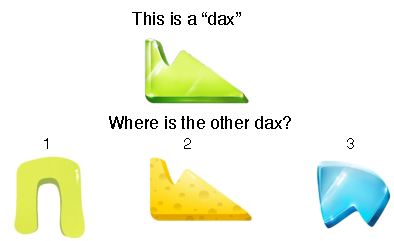
\includegraphics[width=0.35\textwidth]{figures/shape_bias_demo.pdf}
    \end{center}
    \caption{The shape bias. Children learn that objects with the same name
    tend to have the same shape, and thus option 2 above is likely the right
    answer. This inductive bias helps with future word learning.}
    \label{fig:shape_bias_demo}
\end{figure}

If humans extrapolate beyond the presented data, then another source of
information must make up the difference; prior background knowledge must
delimit the hypothesis space during learning \citep{Tenenbaum2011, Lake2017}. By
constraining the space of models considered by the learner, these priors,
referred to herein as ``inductive biases," help the learner make inferences
that go far beyond the observed data. As one manifestation, human children make
use of the shape bias--the assumption that objects that have the same name will
tend to have the same shape--when learning new object names, and thus shape is
more important than color, material and other properties when generalizing a
new label to new examples (Fig. \ref{fig:shape_bias_demo}) \citep{Landau1988}.
Similarly, children assume that object names are mutually exclusive, i.e. that
a novel name probably refers to a novel object rather than a familiar object
\citep{Markman1988}. Although the origin of inductive biases is not always
clear, results show that children, adults and primates can ``learn-to-learn" or
form higher-order generalizations that can improve the efficiency of future
learning \citep{Harlow1949, Smith2002, Dewar2010}.

Cognitive scientists have proposed a number of computational models to explain
how inductive biases are acquired and harnessed for future learning.
Hierarchical Bayesian Models (HBMs) enable probabilistic inference at multiple
levels simultaneously, allowing the model to learn the structure of individual
concepts while simultaneously learning about the structure of concepts in
general (i.e., learning a prior on new concepts)
\citep{Gelman2013, Kemp2007, Salakhutdinov2012}. These models have been used to
explain various forms of ``learning-to-learn" including learning a shape bias
\citep{Kemp2007}, yet it is currently difficult to apply HBMs to the type of
raw, high-dimensional sensory data that children receive, such as images or
audio waves. In some cases, HBMs and related approaches have been applied
successfully to raw high-dimensional data such as when learning handwritten
characters \citep{Lake2015}, but with the help of domain-specific knowledge and
engineering. In contrast, recent progress in training deep neural networks
shows how relatively generic architectures can learn effectively from raw data
\citep{LeCun2015}, providing the potential bridge between controlled simulations
with synthetic data \citep[e.g.,][]{Colunga2005} and large-scale real-world
object recognition tasks with raw data \citep[e.g.,][]{Ritter2017}. Here, we
take advantage of this connection by using neural networks to study
learning-to-learn in several different settings of varying stimulus complexity,
with the goal of isolating the fundamentals of the learning dynamics.

Most related to our work here are studies by \cite{Colunga2005} and
\cite{Ritter2017} investigating neural network accounts of shape bias
development. \cite{Colunga2005} showed that a simple neural network model,
trained via Hebbian learning, can acquire the shape bias when presented with
datasets comparable to human developmental studies. However, these simulations
operate on highly simplified bit-vector data, and it is unclear how their
results generalize to more realistic stimuli. Furthermore, the authors did not
systematically vary the structure of the training set, so we do not know the
exact conditions in which biases arise, nor whether current models are
sufficient to explain it. In a recent study, building on recent advances in
object recognition, \cite{Ritter2017} found that performance-optimized deep
neural networks (DNNs) develop the shape bias over the course of learning when
trained on the popular ImageNet classification dataset consisting of raw
naturalistic images. Although these results highlight an exciting possible
connection between DNNs and developmental psychology, many questions remain.
ImageNet--which contains thousands of labeled examples of each visual
concept--is a poor proxy for human developmental learning sets. Whether or not
these models can acquire the same bias with a training set comparable to humans
remains unknown; an answer to this question may help to explain the
developmental process in children. Furthermore, while the development of the
shape bias is known to predict the onset of vocabulary acceleration in children
\citep{GershkoffStowe2004}, we do not know whether the same holds for DNNs.

We investigate the development and influence of inductive biases in neural
network models using artificial object stimuli designed to closely mimic
developmental studies with human children. Borrowing the experimental paradigm
of \cite{Smith2002}, we evaluate the first- and second-order generalization
capabilities of neural networks trained with variable-sized datasets. Beginning
with simple bit-vector data akin to \cite{Colunga2005}, we systematically vary
the number of categories and the number of exemplars in the training set,
recording generalization performance at each pairing. Parallel experiments are
then performed with RGB image data, where each image consists of a 2D object
with a particular shape, color and texture that is shifted and placed over
white background. For each the bit-vector and RGB image data, we investigate
the parametric relationship between bias strength and attribute similarity in
our models by systematically varying the shape, color and texture attributes of
select test stimuli. Similarly, we evaluate bias strength as a function of
depth in the network. In a final set of experiments, we investigate the
correlation between shape bias acquisition and the rate of concept learning in
our networks, mirroring an analogous study from human developmental psychology
\citep{GershkoffStowe2004}.




\section{Efficient Word Learning}
\label{sec:efficient_learning}
We first set out to model the infant learning tasks described in \cite{Smith2002} using
simple neural networks. In order to do so, we use artificial toy data that is designed
to mimic the training data described in the paper. Each object sample is assigned a shape,
texture and color value. There are two types of model evaluations performed, both drawn from
\cite{Smith2002}.

{\bf1. First-order generalization test}: For the first-order generalization test, infants
are asked to evaluate novel instances of familiar objects. To simulate this test, we train
our neural network models to classify objects, ensuring that objects of the same category
are assigned the same shape. Then, we build a test set by creating one novel exemplar of
each category that appeared in the training set. The novel exemplar has the same
shape as the training exemplars of that category, but a new color and texture combination.
Accuracy is defined as the fraction of test images that are correctly classified by the model.
This test is repeated for different training set sizes, i.e. different combinations of
\{\textit{\# categories}, \textit{\# exemplars}\}. It is important to note that as
\textit{\# categories} increases, the first-order task becomes more difficult.

{\bf2. Second-order generalization test}: For the second-order generalization test, infants
are presented with an exemplar of a novel object category as a baseline. Then, they are
shown 3 comparison objects: one which has the same shape as the baseline, one with the same
color, and one with the same texture. In each case, the other 2 features are different from
the baseline. The infants are asked to select which of the 3 comparison objects are of the
same category as the baseline object. We simulate this test by creating an evaluation set
containing groupings of 4 samples: the baseline, the shape constant, the color constant, and
the texture constant. Each grouping serves as one test example. We find which of the 3
samples the NN thinks to be most similar by evaluating the cosine similarity using the
hidden layer features of the model. Accuracy is defined as the fraction of groupings for
which the model chose the correct (shape-similar) object. This test was repeated for
different training set sizes, i.e. different combinations of \{\textit{\# categories},
\textit{\# exemplars}\}.

\begin{figure*}[h]
    \begin{center}
        % mlp results
        \begin{subfigure}[b]{0.47\textwidth}
            \begin{center}
                % subfigure (a)
                \begin{subfigure}[b]{0.48\textwidth}
                    \begin{center}
                        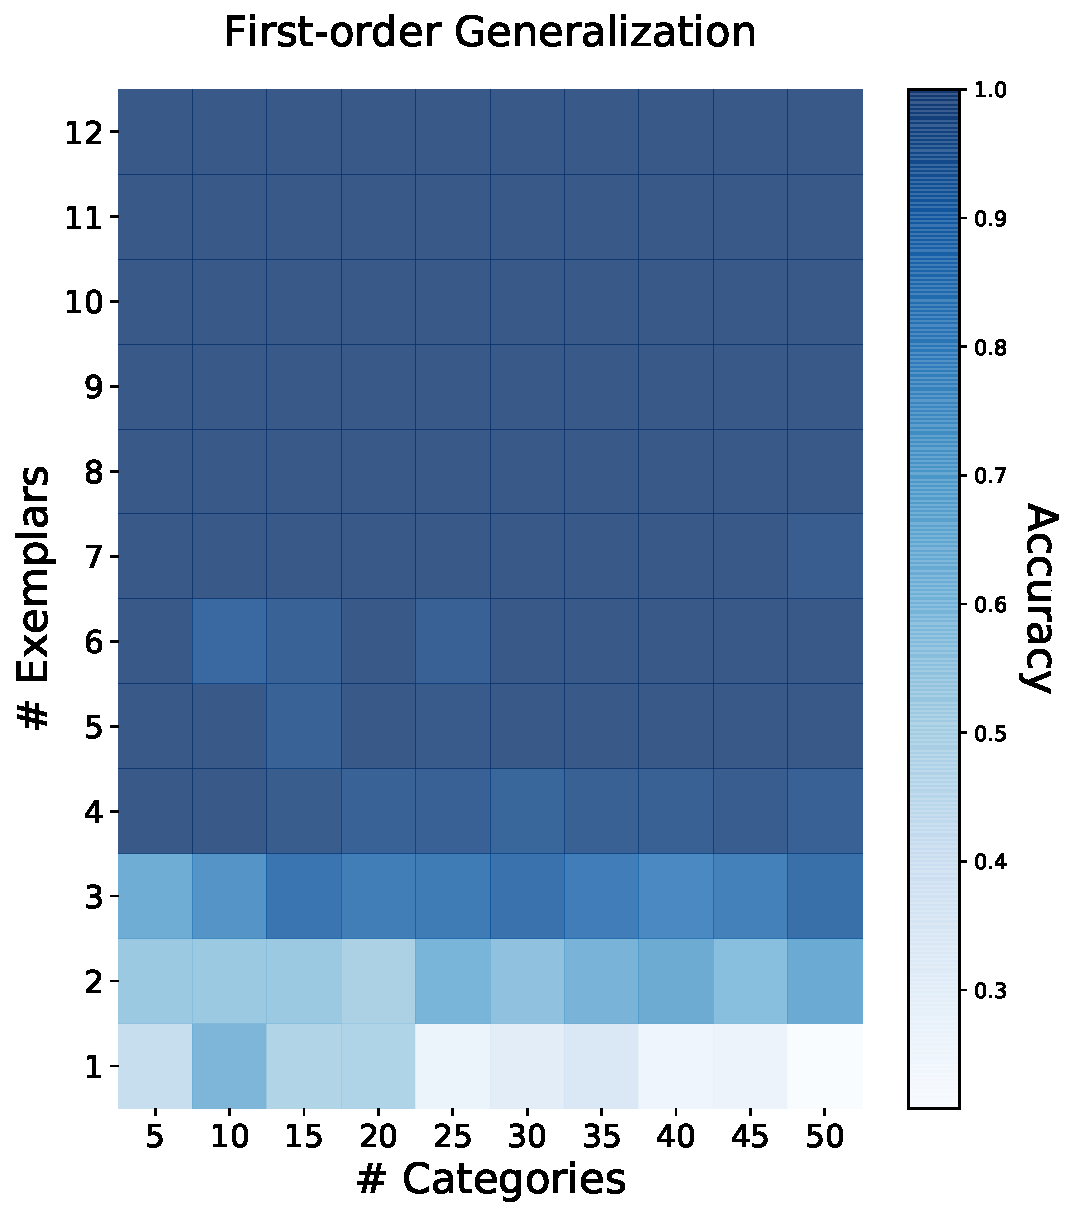
\includegraphics[width=0.98\textwidth]{figures/mlp_1order_accuracy.pdf}
                    \end{center}
                \end{subfigure}
                % subfigure (b)
                \begin{subfigure}[b]{0.48\textwidth}
                    \begin{center}
                        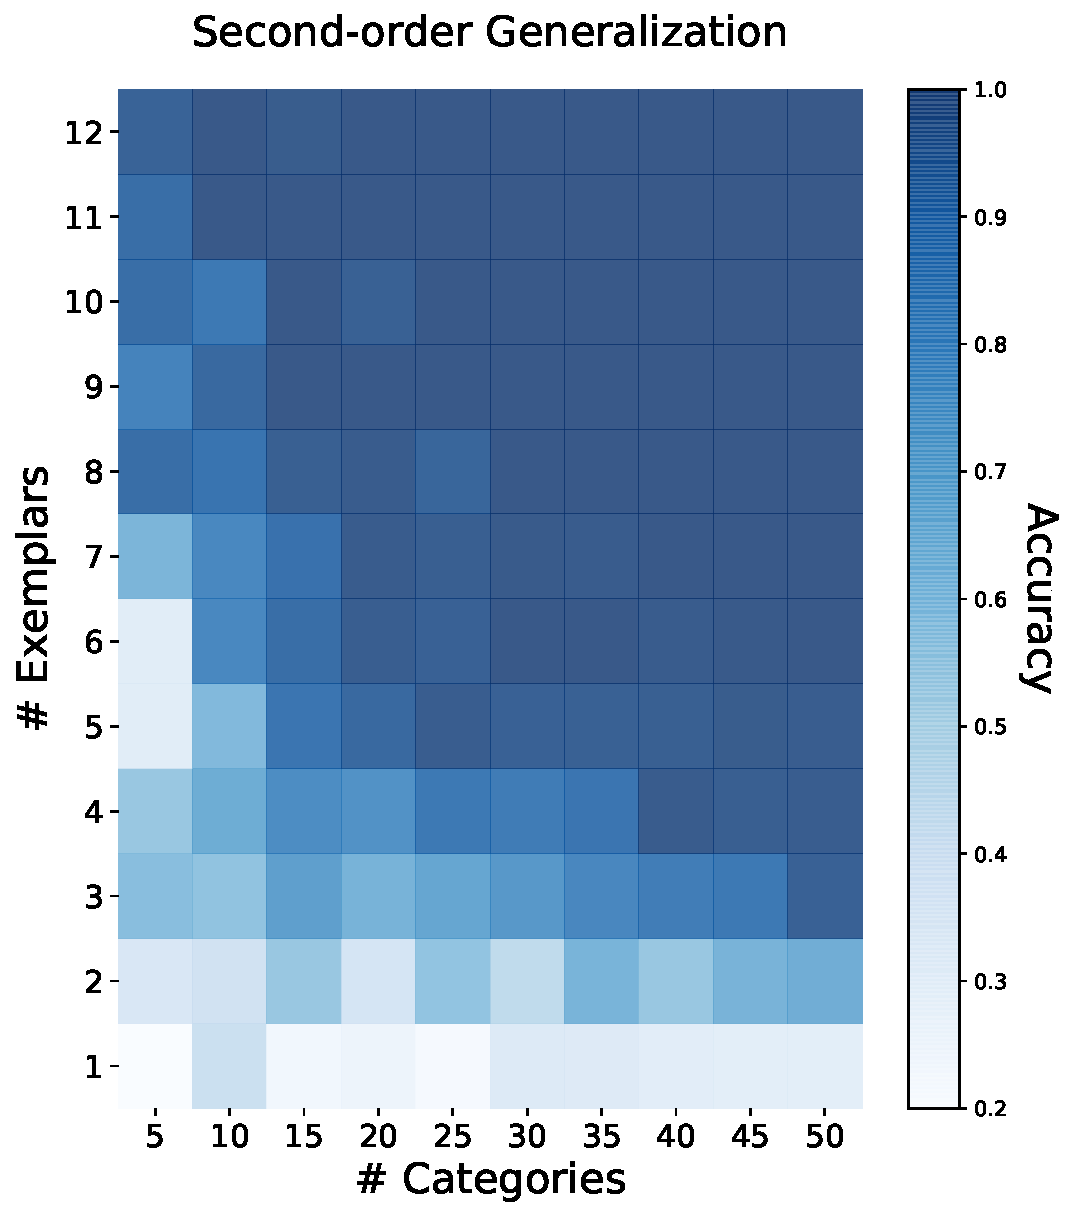
\includegraphics[width=0.98\textwidth]{figures/mlp_2order_accuracy.pdf}
                    \end{center}
                \end{subfigure}
            \end{center}
            \caption{MLP}
            \label{fig:mlp_results}
        \end{subfigure}
        % cnn results
        \begin{subfigure}[b]{0.47\textwidth}
            \begin{center}
                % subfigure (a)
                \begin{subfigure}[b]{0.48\textwidth}
                    \begin{center}
                        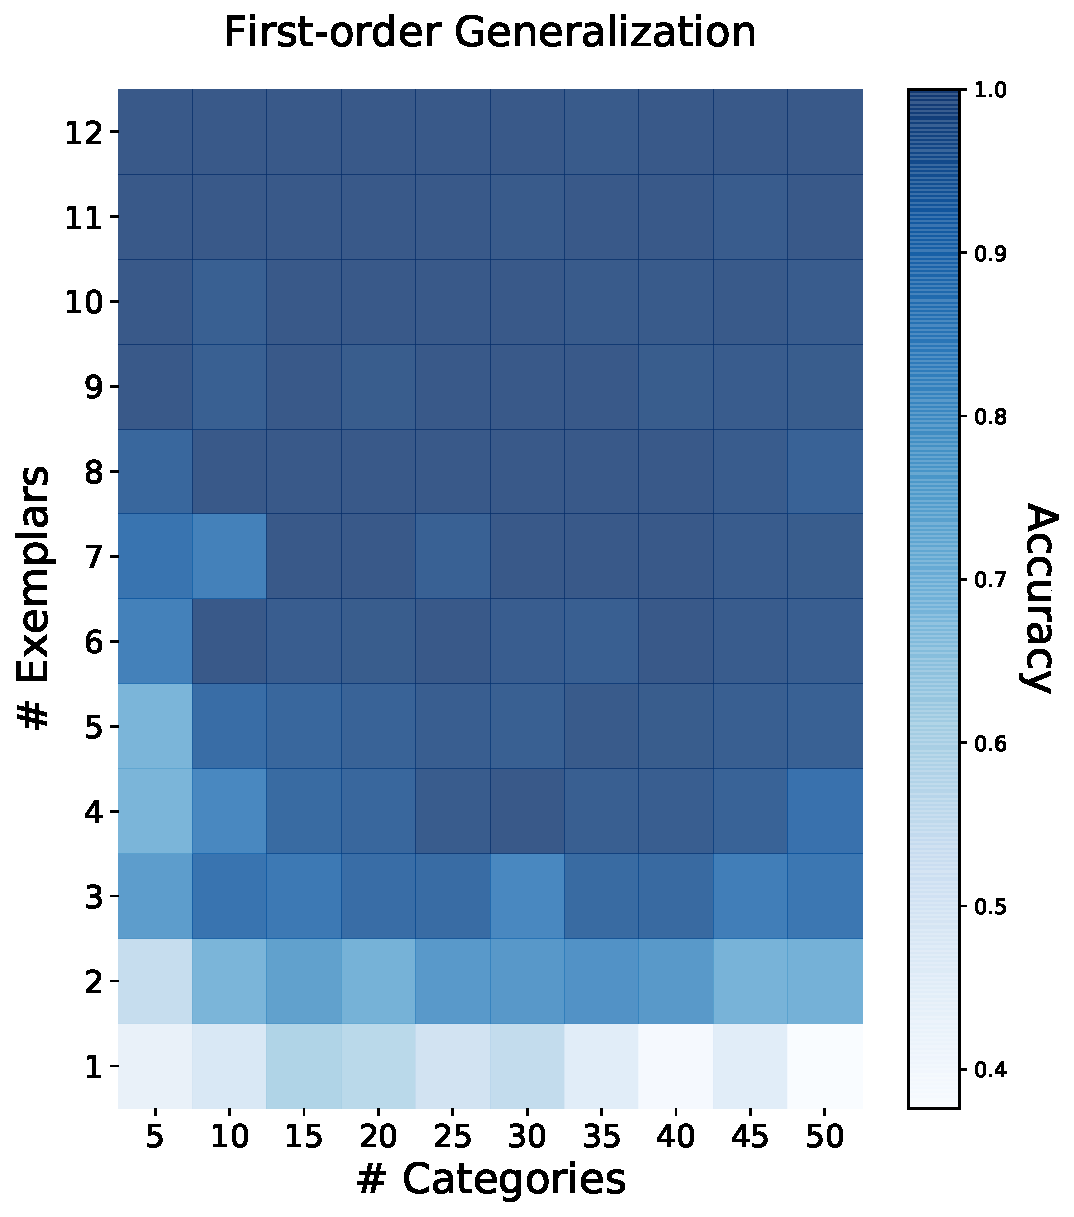
\includegraphics[width=\textwidth]{figures/cnn_1order_accuracy.pdf}
                    \end{center}
                \end{subfigure}
                % subfigure (b)
                \begin{subfigure}[b]{0.48\textwidth}
                    \begin{center}
                        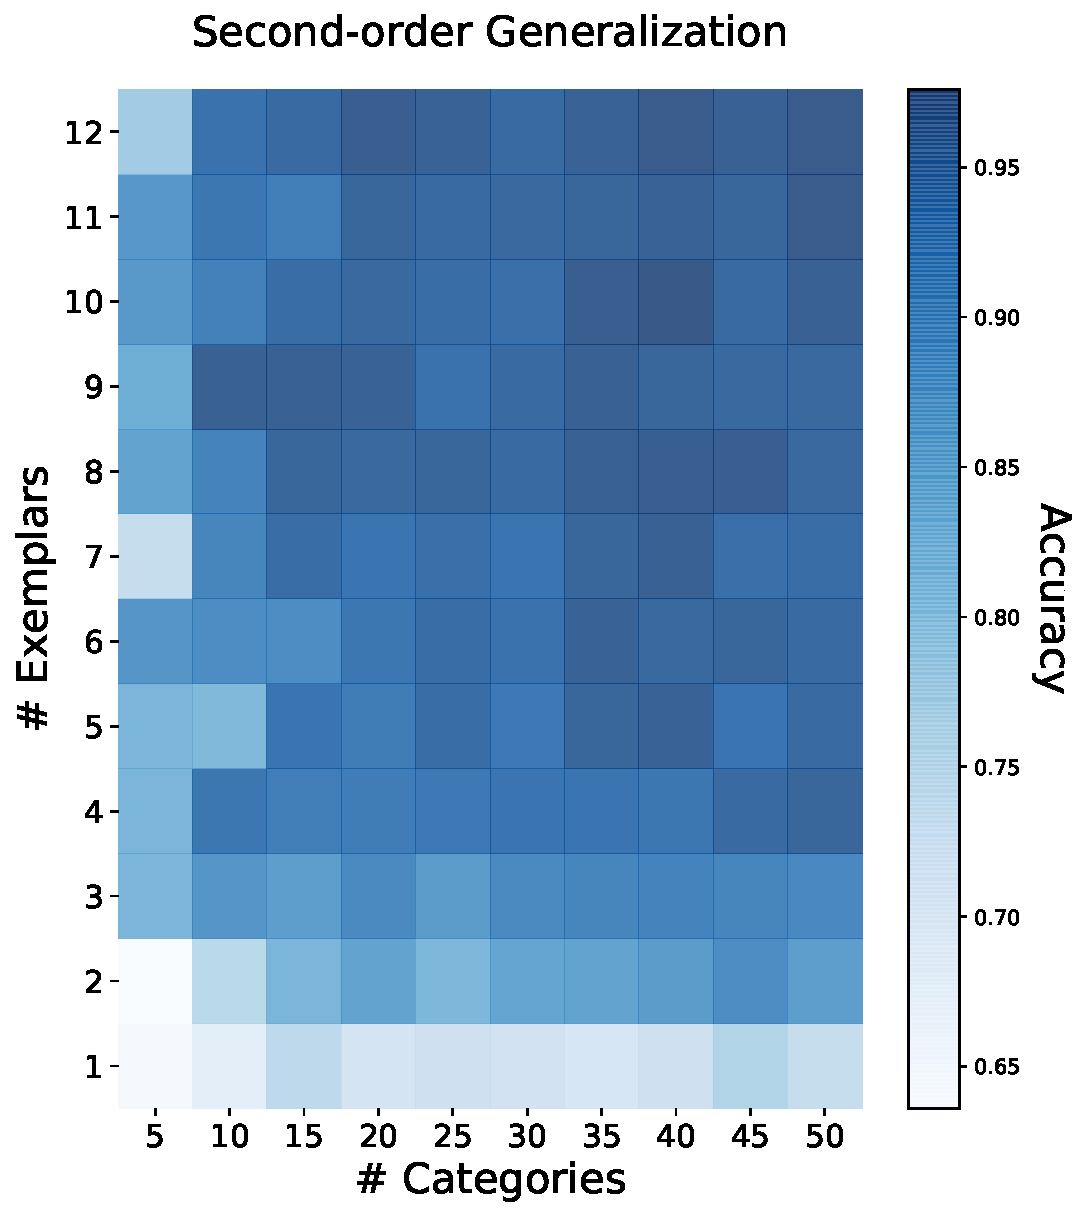
\includegraphics[width=\textwidth]{figures/cnn_2order_accuracy.pdf}
                    \end{center}
                \end{subfigure}
            \end{center}
            \caption{CNN}
            \label{fig:cnn_results}
        \end{subfigure}
    \end{center}
    \caption{First- and second-order generalization results for the simple MLP and CNN models.
    For each \{\textit{\# categories}, \textit{\# exemplars}\} pair, the average result from
    5 trials is shown.}
    \label{fig:generalization_results}
\end{figure*}

\subsection{Simple Multilayer Perceptron}
To begin with, we use a simple multilayer perceptron (MLP) that operates on categorical
data. Since shape, color, \& texture have categorical feature values, we encode the values
using unique bit vectors that are randomly assigned at the beginning of the experiment. We
use a simple feed-forward NN with one hidden layer of 30 units, and the ReLU activation
function. The number of units in the softmax layer depends on the \textit{\# categories}
parameter for the particular dataset. Results are shown in Fig. \ref{fig:mlp_results}.

\subsection{Simple Convolutional Neural Network}
\label{sec:simple_cnn}
As a second type of model, we used a simple convolutional neural network (CNN) architecture
consisting of... TODO. To train this CNN, we generated images of artificial 2-D objects
(Fig. \ref{fig:generated_images}) with a variety of different shape, color and texture values. TODO... finish.
Results are shown in Fig. \ref{fig:cnn_results}.

\begin{figure}[h!]
    \begin{center}
        % shape 1
        \begin{subfigure}[b]{0.3\textwidth}
            \begin{center}
                \begin{subfigure}[b]{0.4\textwidth}
                    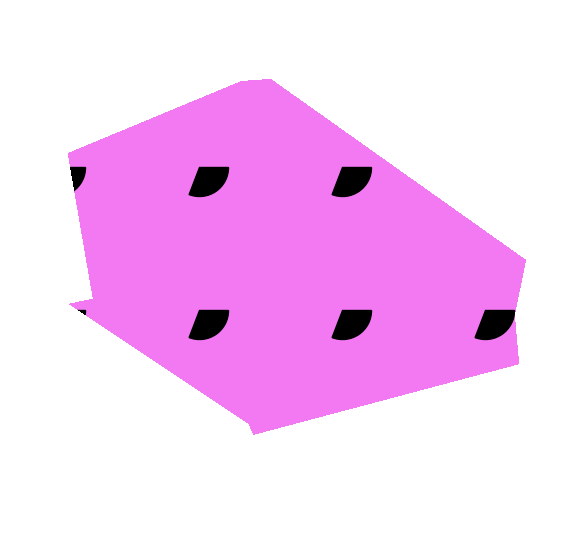
\includegraphics[width=\linewidth]{figures/generated_objects/img0000.png}
                \end{subfigure}
                \begin{subfigure}[b]{0.4\textwidth}
                    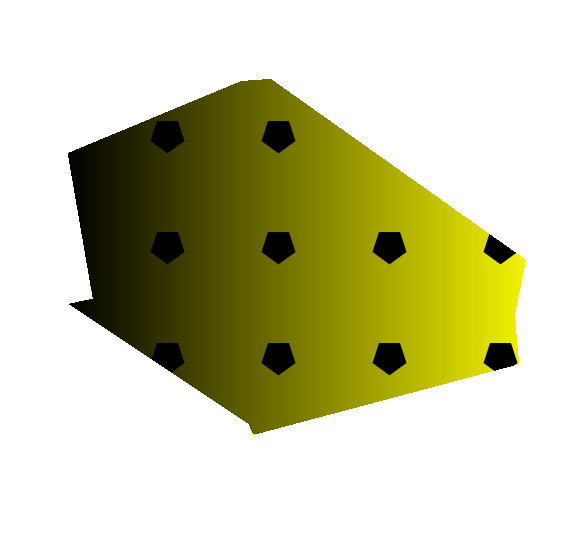
\includegraphics[width=\linewidth]{figures/generated_objects/img0001.png}
                \end{subfigure}
            \end{center}
        \end{subfigure}
        % % shape 2
        \begin{subfigure}[b]{0.3\textwidth}
            \begin{center}
                \begin{subfigure}[b]{0.4\textwidth}
                    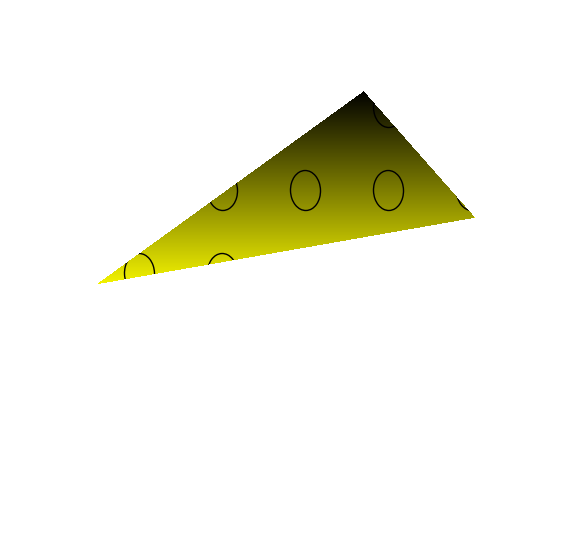
\includegraphics[width=\linewidth]{figures/generated_objects/img0002.png}
                \end{subfigure}
                \begin{subfigure}[b]{0.4\textwidth}
                    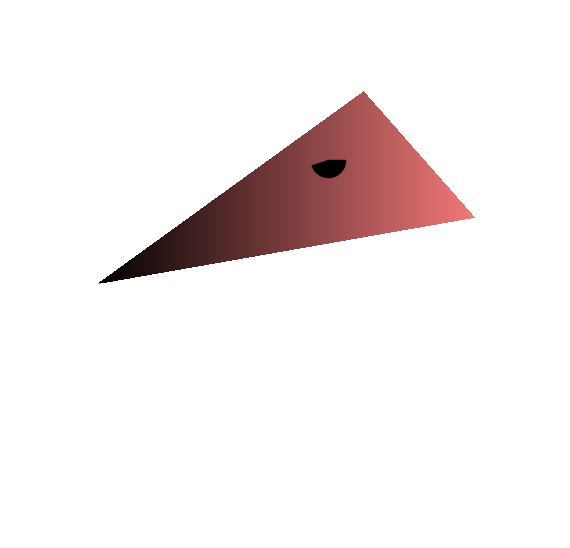
\includegraphics[width=\linewidth]{figures/generated_objects/img0003.png}
                \end{subfigure}
            \end{center}
        \end{subfigure}
        \begin{subfigure}[b]{0.3\textwidth}
            \begin{center}
                \begin{subfigure}[b]{0.4\textwidth}
                    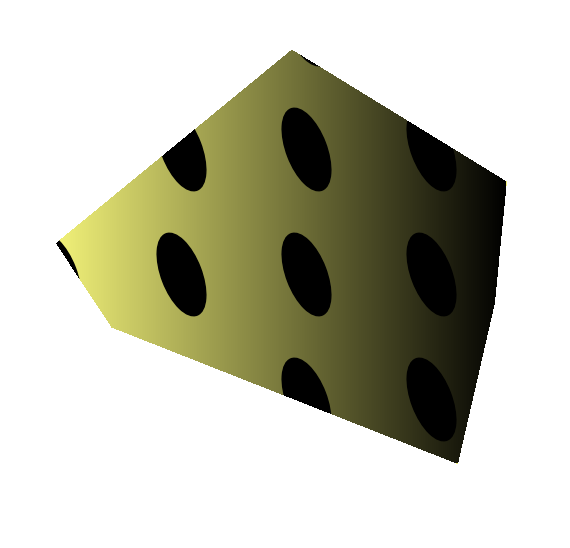
\includegraphics[width=\linewidth]{figures/generated_objects/img0004.png}
                \end{subfigure}
                \begin{subfigure}[b]{0.4\textwidth}
                    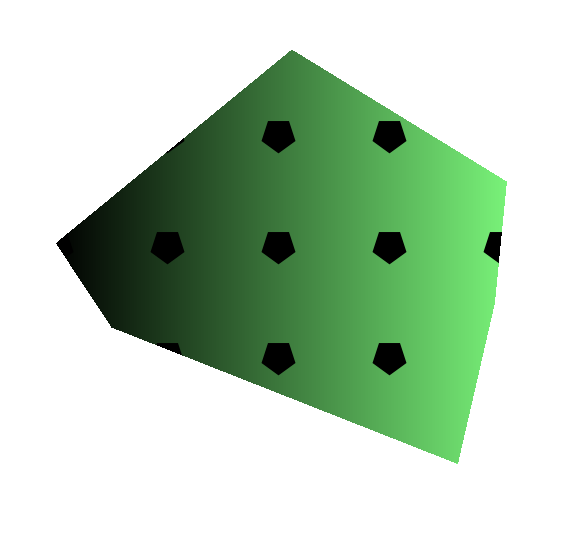
\includegraphics[width=\linewidth]{figures/generated_objects/img0005.png}
                \end{subfigure}
            \end{center}
        \end{subfigure}
    \end{center}
    \caption{Computer-generated images of 2D objects with different shape, color and texture features.}
    \label{fig:generated_images}
\end{figure}

\section{Extensive Bias Analysis}
We next set out to analyze the biases of image classification models in detail. The model that
we choose to investigate is the popular VGG-16 network \cite{}, which has been pre-trained for
the ImageNet classification task.
% In addition to VGG-16, we also investigate the
% biases of our simple CNN from Section \ref{sec:efficient_learning}, trained on artificial objects with dataset
% dimensions \{\}.
Our analysis consists of two parts: 1) a detailed layer-wise investingation of the shape, color and
texture biases, and 2) a parametric analysis of the shape and color biases in these models.

\begin{figure}[h!]
    \begin{center}
        % shape 1
        \begin{subfigure}[b]{0.3\textwidth}
            \begin{center}
                \begin{subfigure}[b]{0.4\textwidth}
                    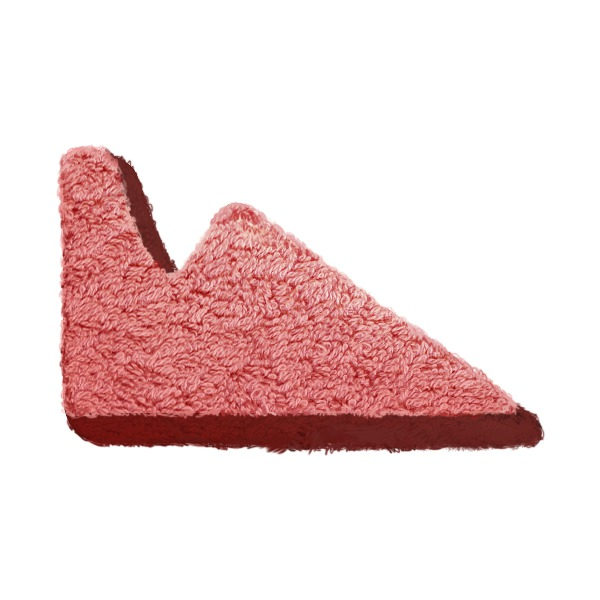
\includegraphics[width=\linewidth]{figures/artist_objects/fake1_carpet_red.jpg}
                \end{subfigure}
                \begin{subfigure}[b]{0.4\textwidth}
                    
\includegraphics[width=\linewidth]{figures/artist_objects/fake1_sponge_yellow.jpg}
                \end{subfigure}
            \end{center}
        \end{subfigure}
        % % shape 2
        \begin{subfigure}[b]{0.3\textwidth}
            \begin{center}
                \begin{subfigure}[b]{0.4\textwidth}
                    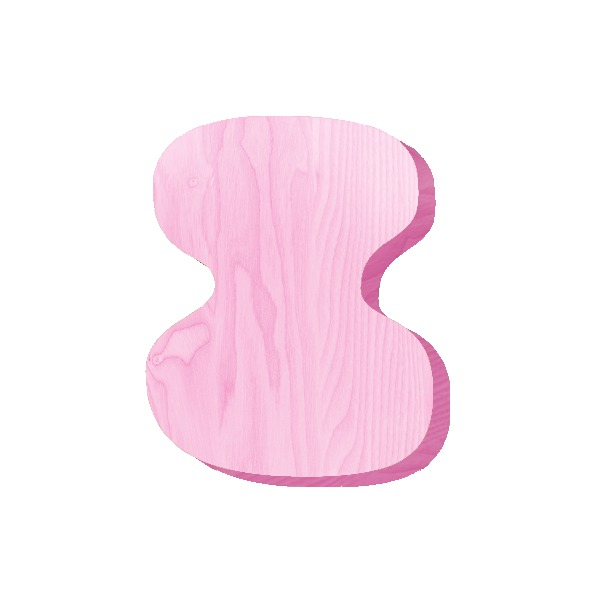
\includegraphics[width=\linewidth]{figures/artist_objects/fake5_wood_pink.jpg}
                \end{subfigure}
                \begin{subfigure}[b]{0.4\textwidth}
                    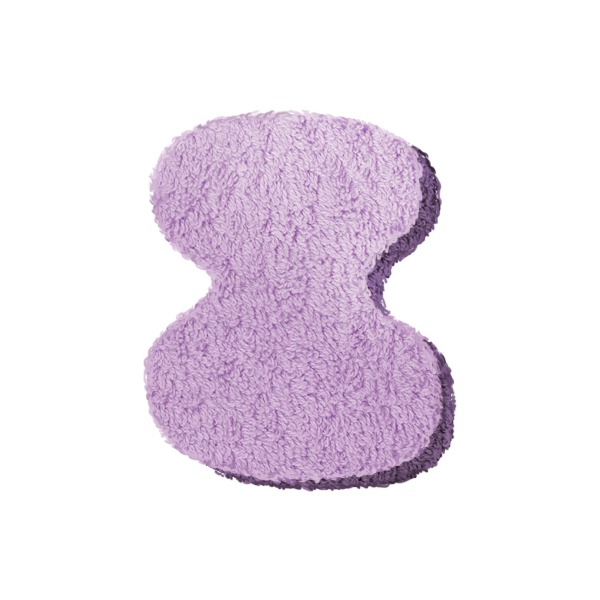
\includegraphics[width=\linewidth]{figures/artist_objects/fake5_carpet_purple.jpg}
                \end{subfigure}
            \end{center}
        \end{subfigure}
        \begin{subfigure}[b]{0.3\textwidth}
            \begin{center}
                \begin{subfigure}[b]{0.4\textwidth}
                    
\includegraphics[width=\linewidth]{figures/artist_objects/fake4_sponge_orange.jpg}
                \end{subfigure}
                \begin{subfigure}[b]{0.4\textwidth}
                    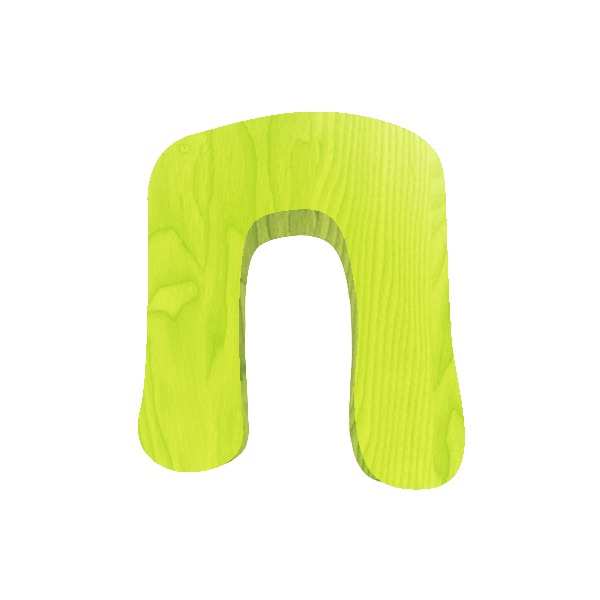
\includegraphics[width=\linewidth]{figures/artist_objects/fake4_wood_green.jpg}
                \end{subfigure}
            \end{center}
        \end{subfigure}
    \end{center}
    \caption{Artist-designed images of 3D objects with different shape, color and texture features.}
    \label{fig:artist_images}
\end{figure}

\begin{figure}[h!]
    \caption{CogPsyc images with different shape, color and texture features (TODO).}
    \label{fig:cogpsyc_images}
\end{figure}

\subsection{Layer-wise Biases}
The first step of our analysis is to evaluate the shape, color and texture biases of VGG-16
at each of its layers, in order to get a picture of how these biases develops along the
higherarchy of the model's internal representation. In order to probe the model, we make
use of two unique image datasets with stimuli that mimic \cite{Smith2002}.

{\bf1. Artist-generated object dataset}: These images were generated by an artist in Adobe
Photoshop. See Fig. \ref{fig:artist_images}.

{\bf2. CogPsyc object dataset}: These images were provided by cognitive psychologist Linda
Smith, and they were used in the experiments of \cite{Ritter2017}. See Fig.
\ref{fig:cogpsyc_images}.

\begin{figure*}[h]
    \begin{center}
        \begin{subfigure}[b]{0.4\textwidth}
            \begin{center}
                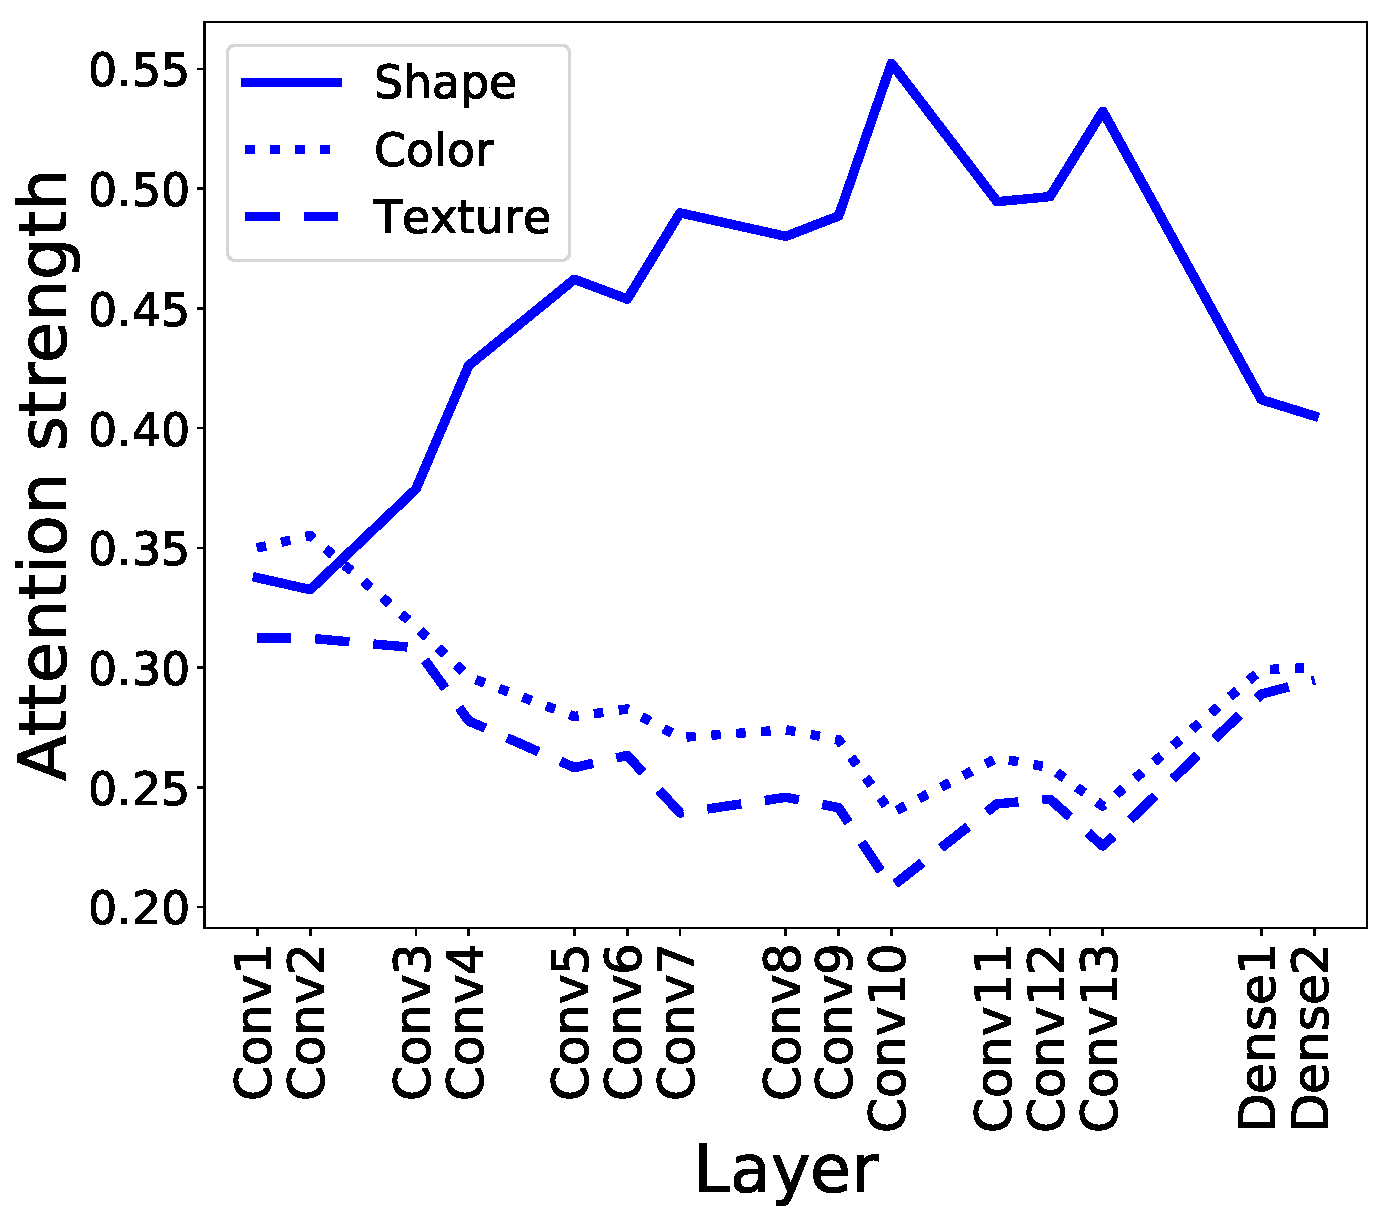
\includegraphics[width=\textwidth]{figures/vgg_layer_biases.pdf}
            \end{center}
            \caption{Artist-generated images}
            \label{fig:biases_artist}
        \end{subfigure}
        \begin{subfigure}[b]{0.4\textwidth}
            \caption{CogPsyc images (TODO)}
        \end{subfigure}
        \caption{VGG-16 layer-wise biases on two image datasets. Attention strength refers to
        the network's similarity score between the target objectand objects that match in
        either shape, color or texture.}
    \end{center}
    \label{fig:layerwise_biases}
\end{figure*}

The layer-wise bias results are shown in Fig. \ref{fig:biases_artist}.

\subsection{Parametric Biases}
The second step of our analysis is to examine how the shape and color biases depend on the intensity
of their respective feature similarities. For these tests, we make use of our computer-generated
images so that we can quantitatively manipulate and evaluate the shape and color features of our
objects. The parametric bias results are shown in Fig. \ref{fig:parametric_others_constant} and
\ref{fig:parametric_others_varying}.
\begin{figure}[h!]
    \begin{center}
        \begin{subfigure}[b]{0.235\textwidth}
            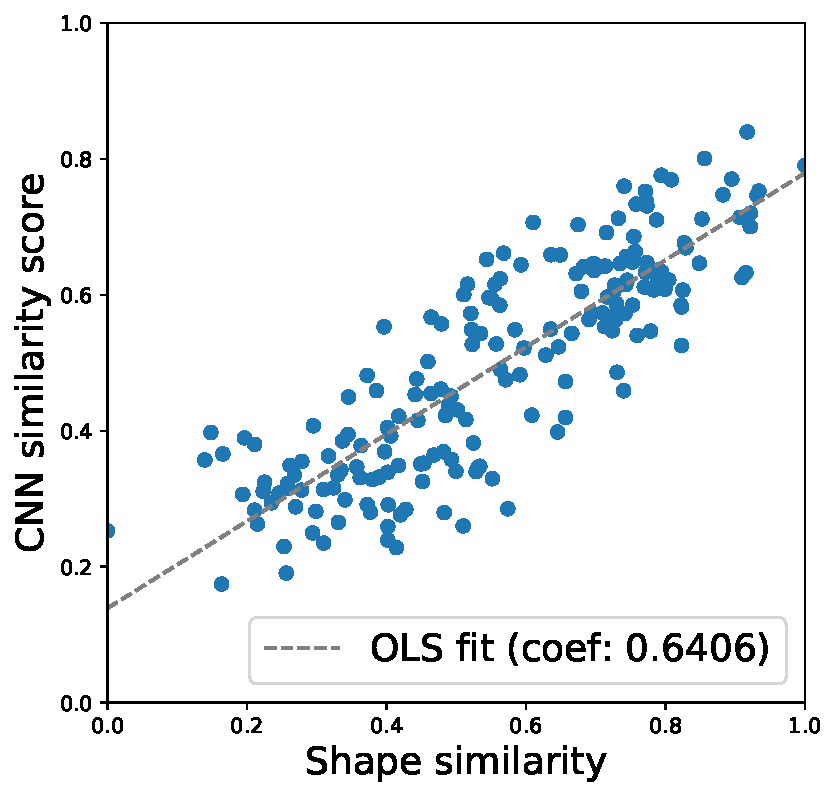
\includegraphics[width=\linewidth]{figures/vgg_shape_parametric_others_constant.pdf}
            \caption{Shape}
        \end{subfigure}
        \begin{subfigure}[b]{0.235\textwidth}
            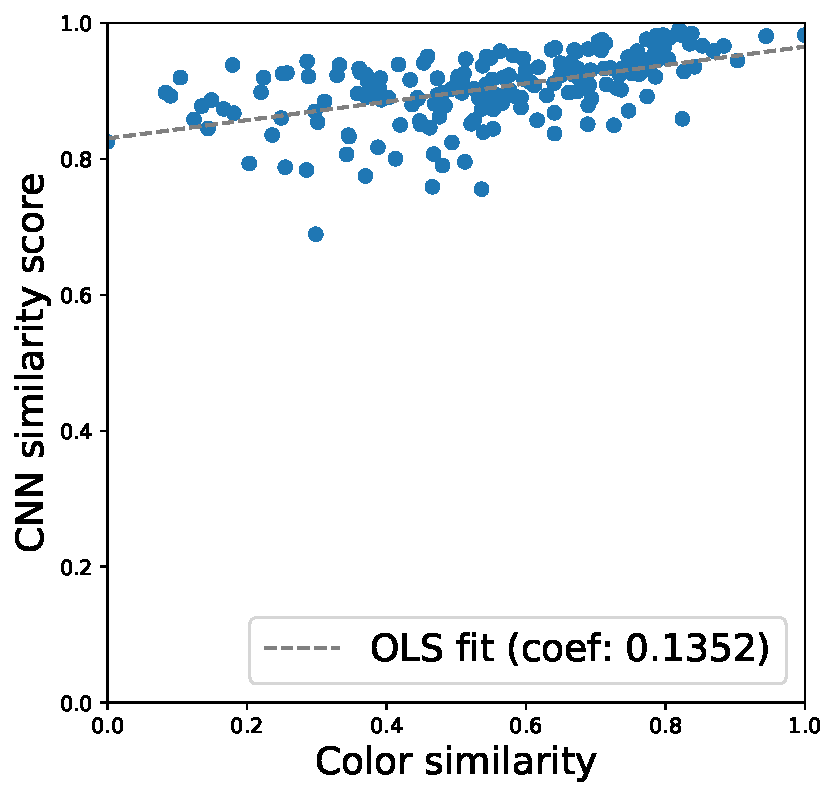
\includegraphics[width=\linewidth]{figures/vgg_color_parametric_others_constant.pdf}
            \caption{Color}
        \end{subfigure}
    \end{center}
    \caption{VGG-16 parametric shape and color biases w/ other features constant.}
    \label{fig:parametric_others_constant}
\end{figure}

\begin{figure}[h!]
    \begin{center}
        \begin{subfigure}[b]{0.235\textwidth}
            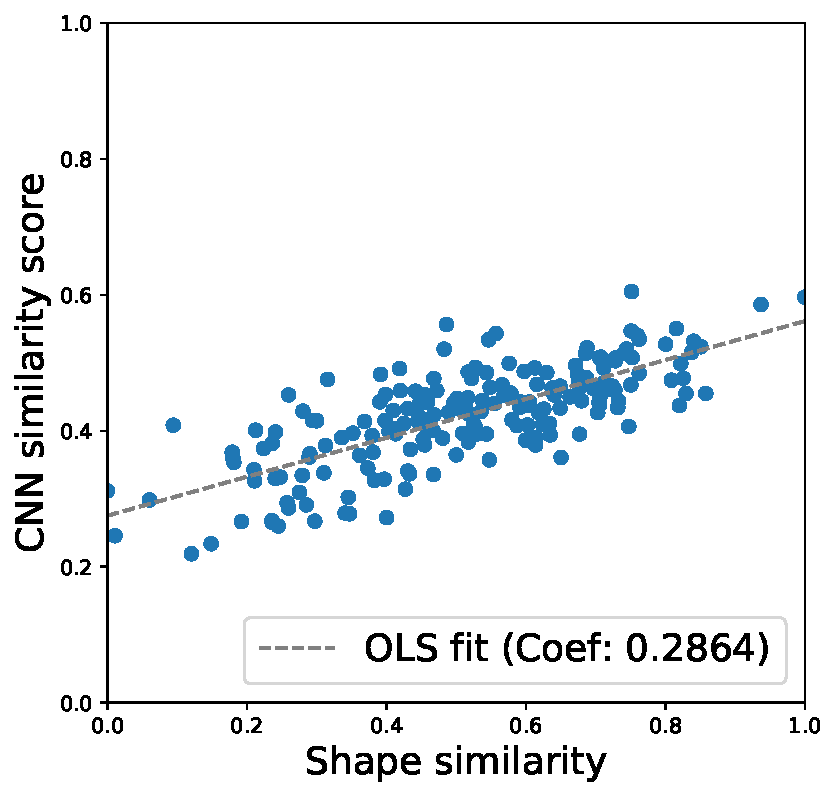
\includegraphics[width=\linewidth]{figures/vgg_shape_parametric.pdf}
            \caption{Shape}
        \end{subfigure}
        \begin{subfigure}[b]{0.235\textwidth}
            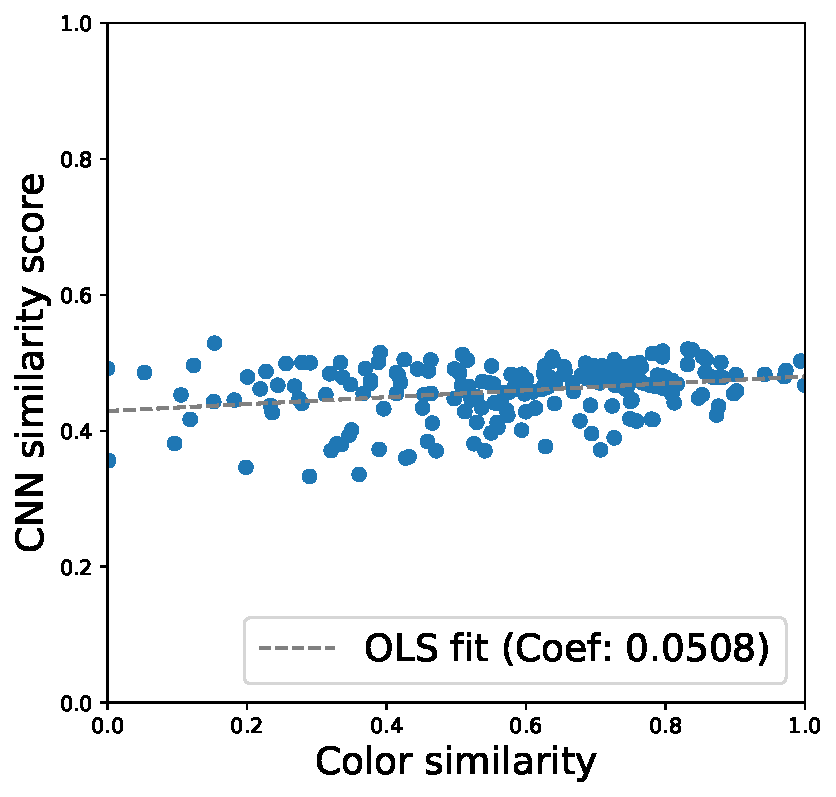
\includegraphics[width=\linewidth]{figures/vgg_color_parametric.pdf}
            \caption{Color}
        \end{subfigure}
    \end{center}
    \caption{VGG-16 parametric shape and color biases w/ other features varying.}
    \label{fig:parametric_others_varying}
\end{figure}

\section{Acknowledgements}

This research was supported by a Henry M. McCracken fellowship and NYU
start-up faculty funding (?). We thank Subhankar Ghosh for useful code and
preliminary experiment ideas.

\nocite{Ritter2017}


\bibliographystyle{apacite}

\setlength{\bibleftmargin}{.125in}
\setlength{\bibindent}{-\bibleftmargin}

\bibliography{citations}


\end{document}
